\begin{figure}
     \centering
     \begin{subfigure}[b]{0.40\textwidth}
         \centering
		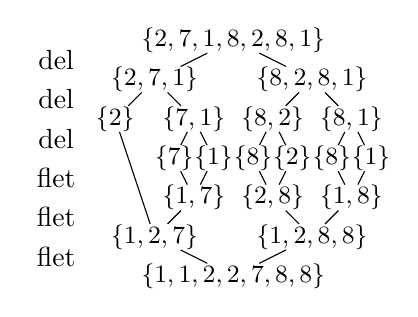
\begin{tikzpicture}[scale =.5,
			s/.style = {font = \small, inner sep = 0pt}]
			\node (2718281) at (-.5,0)  [s] {$\{2,7,1,8,2,8,1\}$};
			\node (1122788) at (-.5,-6) [s] {$\{1,1,2,2,7,8,8\}$};
			\node (271)     at (-2.5,-1)[s] {$\{2,7,1\}$};
			\node (127)     at (-2.5,-5)[s] {$\{1,2,7\}$};
			\node (2)       at (1,-3)   [s] {$\{2\}$};
			\node (2u)      at (-3.5,-2)[s] {$\{2\}$};
			\node (71)      at (-1.5,-2)[s] {$\{7,1\}$};
			\node (17)      at (-1.5,-4)[s] {$\{1,7\}$};
			\node (7)       at (-2,-3)  [s] {$\{7\}$};
			\node (8281)    at (1.5,-1) [s] {$\{8,2,8,1\}$};
			\node (1288)    at (1.5,-5) [s] {$\{1,2,8,8\}$};
			\node (81)      at (2.5,-2) [s] {$\{8,1\}$};
			\node (18)      at (2.5,-4) [s] {$\{1,8\}$};
			\node (1a)       at (-1,-3) [s] {$\{1\}$};
			\node (1b)       at (3,-3)  [s] {$\{1\}$};
			\node (8a)      at (0, -3)  [s] {$\{8\}$};
			\node (8b)      at (2,-3)   [s] {$\{8\}$};
			\node (82)      at (0.5,-2) [s] {$\{8,2\}$};
			\node (28)      at (0.5,-4) [s] {$\{2,8\}$};
			\node at (-5,-0.5) {del};
			\node at (-5,-1.5) {del};
			\node at (-5,-2.5) {del};
			\node at (-5,-3.5) {flet};
			\node at (-5,-4.5) {flet};
			\node at (-5,-5.5) {flet};
			\draw  (2718281) -- (271);
			\draw  (2718281) -- (8281);
			\draw  (271) -- (2u);
			\draw  (271) -- (71);
			\draw  (8281) -- (82);
			\draw  (8281) -- (81);
			\draw  (71) -- (7);
			\draw  (71) -- (1a);
			\draw  (82) -- (8a);
			\draw  (82) -- (2);
			\draw  (81) -- (8b);
			\draw  (81) -- (1b);
			\draw  (8a) -- (28);
			\draw  (2) -- (28);
			\draw  (7) -- (17);
			\draw  (1a) -- (17);
			\draw  (8b) -- (18);
			\draw  (1b) -- (18);
			\draw  (2u) -- (127);
			\draw  (17) -- (127);
			\draw  (28) -- (1288);
			\draw  (18) -- (1288);
			\draw  (127) -- (1122788);
			\draw  (1288) -- (1122788);
		\end{tikzpicture}
         \caption{$y=x$}
         \label{fig:y equals x}
     \end{subfigure}
     \hfill
     \begin{subfigure}[b]{0.55\textwidth}
         \centering
		\begin{tabular}{rrl|l}
			$a$ & $b$ & $c$ & Operation\\
			\hline
			$\{1,2,7\}$ &$ \{1,2,8,8\}$ &  $ \{\,\}$ & flyt fra $a$\\
			$\{2,7\}$ &$ \{1,2,8,8\}$ &  $ \{1\}$ & flyt fra $b$\\
			$\{2,7\}$ &$ \{2,8,8\}$ &  $ \{1,1\}$ & flyt fra $a$\\
			$\{7\}$ &$ \{2,8,8\}$ &  $ \{1,1,2\}$ & flyt fra $b$\\
			$\{7\}$ &$ \{8,8\}$ &  $ \{1,1,2,2\}$ & flyt fra $a$\\
			$\{\,\}$ &$ \{8,8\}$ &  $ \{1,1,2,2,7\}$ & sammenføj $b$\\
			$\{\,\}$ &$ \{\,\}$ &  $ \{1,1,2,2,7,8,8\}$ & \\
		\end{tabular}
         \caption{$y=3sinx$}
         \label{fig:three sin x}
     \end{subfigure}
	\caption{Hvordan mergesort først opdeler, og derefter samler listen. \cite[s. 106]{aogd}}
	\label{fig:mergesort_procedure}
\end{figure}
